\documentclass[twoside,11pt]{article}

% Any additional packages needed should be included after jmlr2e.
% Note that jmlr2e.sty includes epsfig, amssymb, natbib and graphicx,
% and defines many common macros, such as 'proof' and 'example'.
%
% It also sets the bibliographystyle to plainnat; for more information on
% natbib citation styles, see the natbib documentation, a copy of which
% is archived at http://www.jmlr.org/format/natbib.pdf

\usepackage{csc498project}
\usepackage{url}
\usepackage{graphicx}
\graphicspath{ {./images/} }
\usepackage{float}

\newcommand\fnurl[2]{%
  \href{#2}{#1}\footnote{\url{#2}}%
}

% Short headings should be running head and authors last names

\ShortHeadings{Atari Breakout Reinforcement Learning Environment}{Your names}
\firstpageno{1}


\title{Atari Breakout Reinforcement Learning Environment}

\author{\name Haider Sajjad \email haider.sajjad@mail.utoronto.ca \\
       \addr 1004076251\\
       \AND
      \name Weiyu Li \email weiyu.li@mail.utoronto.ca \\
       \addr 1003765981}

\begin{document}

\maketitle

\begin{abstract}%   <- trailing '%' for backward compatibility of .sty file
\textit{
Atari Breakout environment implementation and training an agent using multiple algorithms over a generated environment (changing brick layouts)}

\end{abstract}

\section{Introduction}
Our project is implementing an Atari breakout environment and training an agent to play it across general levels. The project repository can be found here: \url{https://github.com/duoduocai-dot/csc498-project} To play the original game, after cloning the project, just run the file \fnurl{run\_Breakout.py}{https://github.com/duoduocai-dot/csc498-project/blob/main/run_Breakout.py}.\\
Our environment is \fnurl{here}{https://github.com/duoduocai-dot/csc498-project/blob/main/breakout.py}. We made a made our environment embedded into a pygame class for Breakout, adding environment functions and variables. \\
We made 6 algorithms which play Breakout, and compare their performance in this report. The algorithms we made are: DQN, double-DQN, policy gradient REINFORCE, tabular Q-Learning, tabular double Q-Learning, and tabular SARSA.

\section{Environment}
Our environment is here: \url{https://github.com/duoduocai-dot/csc498-project/blob/main/breakout.py}.
\subsection{Rewards}
We experimented with various reward mechanisms. Our original reward schema was:
\begin{itemize}
\item +10 for ball hitting paddle
\item -10 ball missing paddle
\item +1 ball hits brick
\item -0.2 movement penalty
\item +1000 ball destroys all bricks
\end{itemize}
However, with this model we noticed it was difficult for the agent to actually learn, as it doesn't get direct feedback after making an action. So we altered the reward schema to be:
\begin{itemize}
\item +10 for ball hitting paddle
\item -10 ball missing paddle
\item \fnurl{Distance between paddle and ball in the x-Axis}{https://github.com/duoduocai-dot/csc498-project/blob/main/breakout.py\#L179}
\item +1000 ball destroys all bricks
\end{itemize}
\subsection{Environment variables, functions} 
Regarding the rest of the environment, the step function is \fnurl{here}{https://github.com/duoduocai-dot/csc498-project/blob/f46268a6c9241b77efd6c96a6dd8ecc3ec5bae1e/breakout.py\#L266}, where the paddle moves depending on the action passed in, and updates rewards for that step. It then returns the game state which is \fnurl{[paddle x-location, ball x-location, ball y-location,ball x-speed, ball y-speed, bricks left]}{https://github.com/duoduocai-dot/csc498-project/blob/f46268a6c9241b77efd6c96a6dd8ecc3ec5bae1e/breakout.py\#L246}.
\\
The \href{https://github.com/duoduocai-dot/csc498-project/blob/f46268a6c9241b77efd6c96a6dd8ecc3ec5bae1e/breakout.py#L299}{reset} function resets the environment, setting ball, bricks, paddle to their original position. 
\\ \href{https://github.com/duoduocai-dot/csc498-project/blob/f46268a6c9241b77efd6c96a6dd8ecc3ec5bae1e/breakout.py#L316}{Render} function, renders the game. \href{https://github.com/duoduocai-dot/csc498-project/blob/f46268a6c9241b77efd6c96a6dd8ecc3ec5bae1e/breakout.py#L332}{The make} function creates the brick layout, and \href{https://github.com/duoduocai-dot/csc498-project/blob/f46268a6c9241b77efd6c96a6dd8ecc3ec5bae1e/breakout.py#L335}{main function} allows a player to play the game. 
\\
Agent actions are to \href{https://github.com/duoduocai-dot/csc498-project/blob/f46268a6c9241b77efd6c96a6dd8ecc3ec5bae1e/breakout.py#L270}{move left (0), move right (1), stay still (2)}.
\\
There is more about the environment including the \href{https://github.com/duoduocai-dot/csc498-project/blob/f46268a6c9241b77efd6c96a6dd8ecc3ec5bae1e/breakout.py#L55}{brickLayout} which we used in testing and comparing the tabular algorithms which will be talked about in it's own section.  

\section{Algorithims}

\subsection{Tabular Algorithms}
We made 3 algorithms which utilize a tabular setup. To discretize the problem, we reduced the state sizes such that they could fit inside a table.
\\\\
How we created the tabular setup is by first getting every possible paddle and ball locations
using this \fnurl{discretizeStateSpaceAllStates function}{https://github.com/duoduocai-dot/csc498-project/blob/main/tabular_Q_learning.py\#L223} which splits the paddle x-locations into 20 possible locations, the ball x-locations into 80 possible locations, and ball y-locations into 30 possible locations. The game screen is 800x600 and paddle is 80 wide and ball is 5x5.
\\\\
We experimented with 3 different schemas to discretize the state space. These included:
\begin{itemize}
\item \href{https://github.com/duoduocai-dot/csc498-project/blob/main/tabular_Q_learning.py#L180}{10 paddle locations, 40 ball x-locations, 20 ball y-locations}
\item \href{https://github.com/duoduocai-dot/csc498-project/blob/main/tabular_Q_learning.py#L203}{10 paddle locations, 80 ball x-locations, 30 ball y-locations}
\item \href{https://github.com/duoduocai-dot/csc498-project/blob/main/tabular_Q_learning.py#L223}{20 paddle locations, 80 ball x-locations, 30 ball y-locations}
\end{itemize}
The last one with the most paddle and ball locations worked best:
\begin{figure}[H]
Rewards from the last 10 episodes using fewest number of states (first bullet):\\
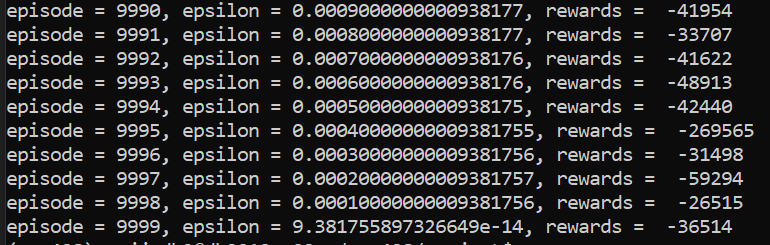
\includegraphics[scale=0.5]{rewards_last_10_episodes_fewest_number_states}
\centering
\end{figure}
\begin{figure}[H]
Rewards from the last 10 episodes using largest number of states (last bullet):\\
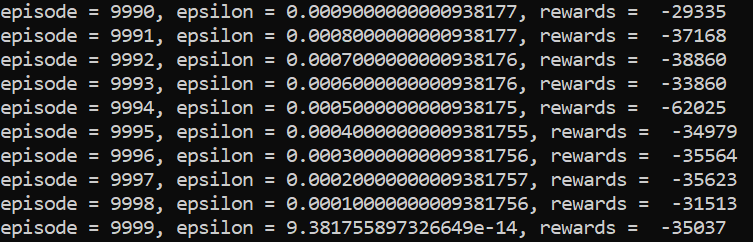
\includegraphics[scale=0.5]{rewards_last_10_episodes_largest_number_states}
\centering
\\ It's clear that the larger number of states gives more rewards.
\end{figure}
After, we \href{https://github.com/duoduocai-dot/csc498-project/blob/main/tabular_Q_learning.py#L37}{create dictionaries to store the policy and Q-values}, with every possible state using the schema above.

\subsubsection{\href{https://github.com/duoduocai-dot/csc498-project/blob/main/tabular_Q_learning.py}{Tabular Q-Learning}}
For tabular Q-Learning, now with a table of all possible states, we can just apply the Q-Learning epsilon greedy algorithm. Where the Q-Learning step is:
\begin{equation}
Q(s_t,a_t) \leftarrow Q(s_t,a_t) + \alpha (r_t + \gamma max_a Q(s_{t+1},a) - Q(s_t,a_t))
\end{equation}

This exact Q-Learning update can be found \href{https://github.com/duoduocai-dot/csc498-project/blob/main/tabular_Q_learning.py#L90}{here}. Where we get the Q-value at each action for the next state, and plug in the max Q-value for the next state into the equation.
\\\\
The other important aspect of Q-Learning is the epsilon-greedy exploration. We first initialize our \href{https://github.com/duoduocai-dot/csc498-project/blob/main/tabular_Q_learning.py#L54}{epsilon in the class}, then it is updated after every \href{https://github.com/duoduocai-dot/csc498-project/blob/main/tabular_Q_learning.py#L285}{episode}. 
\\
Regarding epsilon decay, to increase exploitation rather than exploration, instead of the usual $\epsilon = \epsilon/k$ approach, \href{https://github.com/duoduocai-dot/csc498-project/blob/main/tabular_Q_learning.py#L285}{we use $\epsilon = \epsilon + decay$ where decay} is some negative number between 0 and 1.

\subsubsection{\href{https://github.com/duoduocai-dot/csc498-project/blob/main/tabular_double_Q_learning.py}{Tabular Double Q-Learning}}
In tabular double Q-Learning, our \href{https://github.com/duoduocai-dot/csc498-project/blob/main/tabular_double_Q_learning.py}{algorithm} is nearly the exact same as tabular Q-Learning, except we maintain \href{https://github.com/duoduocai-dot/csc498-project/blob/main/tabular_double_Q_learning.py#L40}{two} Q-value dictionaries and each one is updated with 0.5 \href{https://github.com/duoduocai-dot/csc498-project/blob/main/tabular_double_Q_learning.py#L91}{probability}.
Pseudocode for double Q-Learning:
\\
Select $a_t$ using epsilon greedy $\pi(s) = argmax_a Q_1(s_t, a)+Q_2(s_t, a)$ 
\\
with 0.5 probability:
\begin{equation}
Q_1(s_t,a_t) \leftarrow Q_1(s_t,a_t) + \alpha (r_t + \gamma Q_1(s_{t+1}, argmax_a Q_2(s_{t+1},a)) - Q_1(s_t,a_t))
\end{equation}
else:
\begin{equation}
Q_2(s_t,a_t) \leftarrow Q_2(s_t,a_t) + \alpha (r_t + \gamma Q_2(s_{t+1}, argmax_a Q_1(s_{t+1},a)) - Q_2(s_t,a_t))
\end{equation}


\subsubsection{\href{https://github.com/duoduocai-dot/csc498-project/blob/main/Sarsa.py}{Tabular Sarsa}}
The only thing different from the tabular SARSA implementation from the above two, is that the Q-value update is done using a \fnurl{bootstrapped one-step look ahead}{https://github.com/duoduocai-dot/csc498-project/blob/main/Sarsa.py\#L80}, like in the equation:
\begin{equation}
Q(s_t,a_t) \leftarrow Q(s_t,a_t) + \alpha (r_t + \gamma Q(s_{t+1},a_{t+1}) - Q(s_t,a_t))
\end{equation}

\subsubsection{Training} 
To train each of the algorithms, there is a training function which creates an instance of the algorithm then loops through a number of episodes collecting states, actions and rewards and using them for training. The code to run the training is in \fnurl{tabular\_experiments.py}{https://github.com/duoduocai-dot/csc498-project/blob/main/tabular_experiments.py\#L130}

\subsection{Tabular algorithms Analysis} 
\subsubsection{Performance}
All 3 tabular algorithms do achieve good performance and are able to play the game effectively.
\\\\
Here are graphs for all 3 algorithms, it's clear that as episodes increase and epsilon grows smaller, all 3 algorithms achieve higher rewards. These graphs were made using the \href{https://github.com/duoduocai-dot/csc498-project/blob/main/tabular_experiments.py#L125}{experiment2 function in tabular\_experiments.py}. All three algorithms were trained for 40000 episodes 21000 steps each, with a decay value of -0.000026 as specified in the experiment function. They were all trained on brick-layout 1 (the one with the spaces between bricks, check brick-layout section) The bottom left graph is Q-Learning, top is double Q-Learning, and bottom right is SARSA. Each algorithm took approximately 5-6 hours to train with the above episodes and steps. Also the y-axis is on a scale of $10^6$ for DQL and SARSA and $10^7$ for QL.
\begin{figure}[H]
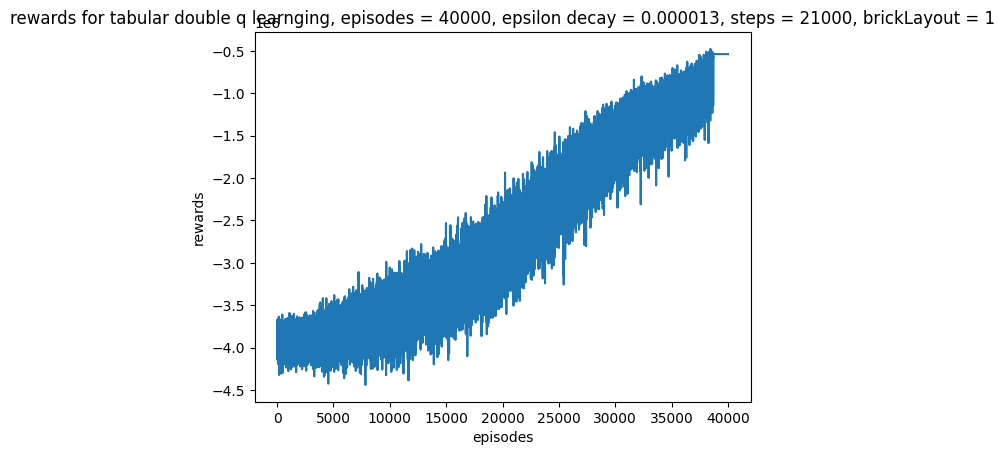
\includegraphics[scale=0.4]{Rewards_Double_Q_Learning}
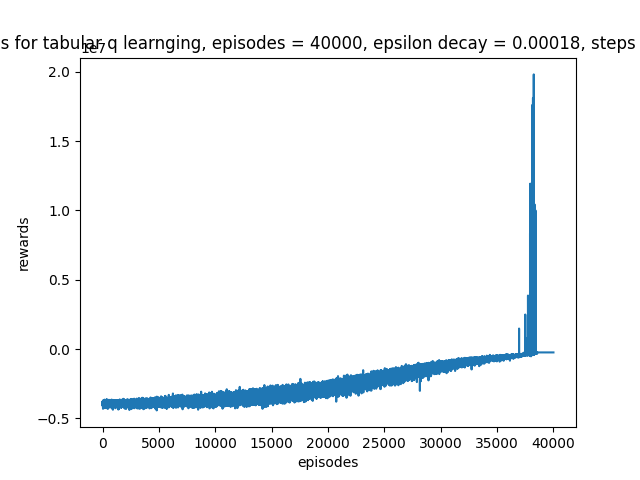
\includegraphics[scale=0.4]{Rewards_Q_Learning}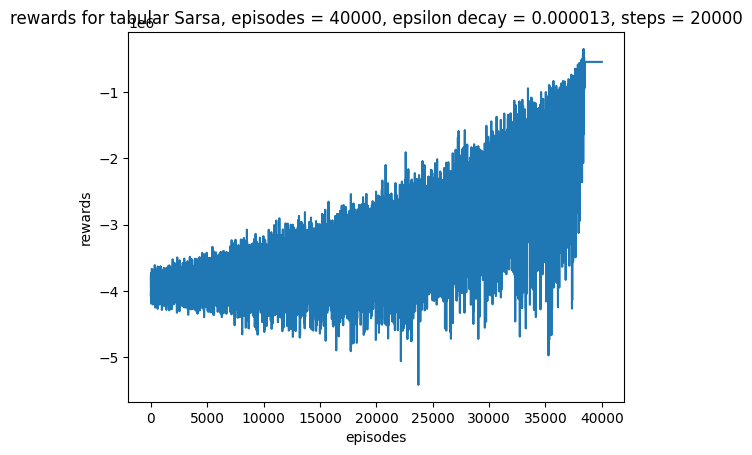
\includegraphics[scale=0.4]{Rewards_Sarsa}
\centering
\end{figure}


\subsubsection{\href{https://github.com/duoduocai-dot/csc498-project/blob/main/tabular_experiments.py\#L10}{Comparing Tabular Algorithms}}
Here is a direct comparison of all 3 algorithms trained over 10000 episodes for 5000 steps per. It's clear from the pictures that Q-Learning and double Q-Learning outpreform SARSA. First graph is full rewards comparison over all episodes, second is over the last 3000 episodes:
\begin{figure}[H]
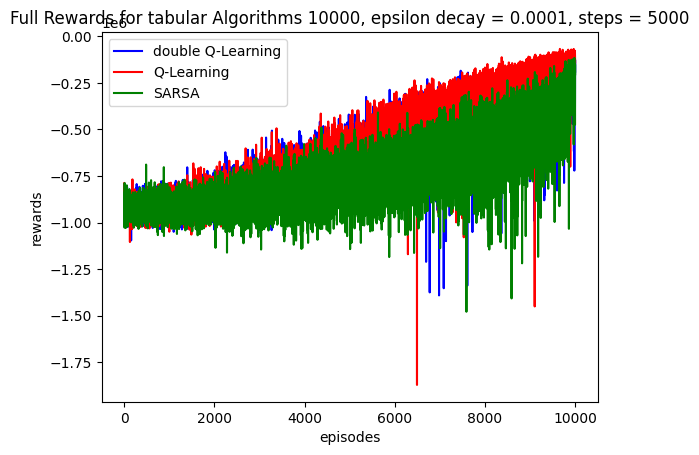
\includegraphics[scale=0.3]{Full_Rewards_Comparison1}
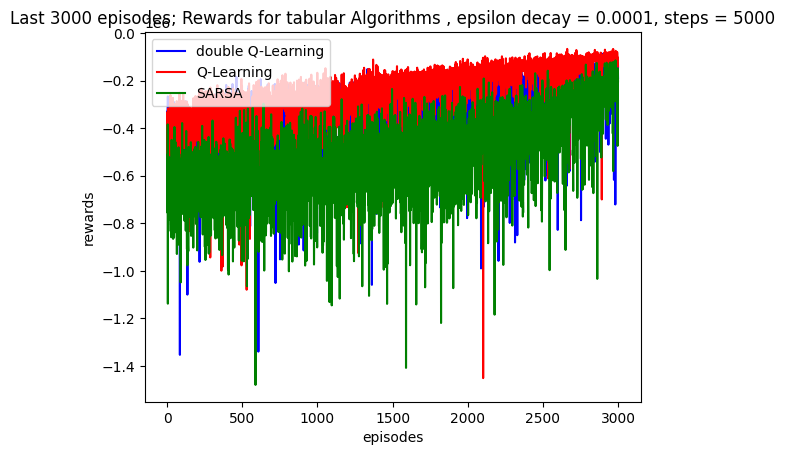
\includegraphics[scale=0.3]{Last_3000_rewards_comparison1}
\centering
\end{figure}


\subsubsection{Parameter and Hyperparameter Choice}
In the tabular algorithms there were many parameters that we used: epsilon and decay-value, episodes, step size, learning rate ($\alpha$),  discount ($\gamma$).
\\\\
The choice of epsilon was simply just 1. We wanted lots of exploration in the beginning, for the agent to learn the environment. The epsilon decay was implemented such that: $\epsilon = \epsilon + decay$. The reason for this is because we wanted a linear decrease of epsilon to account for lots of exploration. 
\\\\
Our choice of step size to fully complete the game is 20000. The reason for the large step size is that the game overall takes a long time to complete. For example, this \fnurl{video example}{https://github.com/duoduocai-dot/csc498-project/blob/main/pictures_and_videos/tabular_double_q_learning_example.mkv} of a double Q-Learning agent playing the game takes more than 30000 steps.
\\\\
Our choice of $\gamma$ was 0.9 because we wanted the agent to count future states heavily because it takes many steps for the agent to win the game, and we wanted to account for this with our discount.
\subsubsection{Q-Learning maximization problems}
We had maximization bias occur in our Q-Learning agents:
\begin{figure}[H]
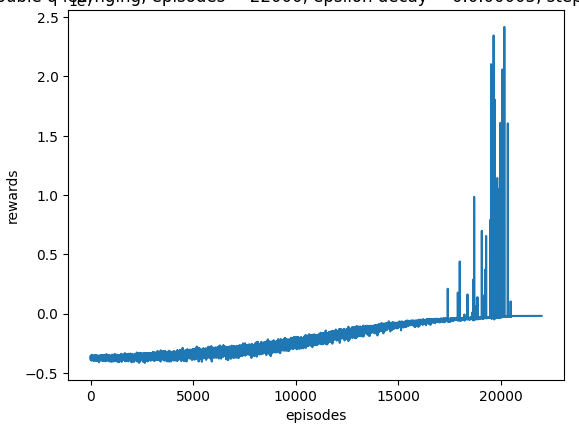
\includegraphics[scale=0.4]{Rewards_Double_Q_Learning_7}
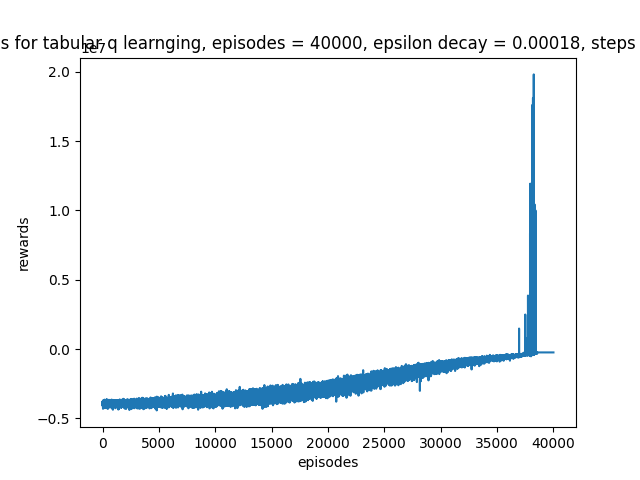
\includegraphics[scale=0.4]{Rewards_Q_Learning}
\centering
\end{figure}
This is an \fnurl{example video}{https://github.com/duoduocai-dot/csc498-project/blob/main/pictures_and_videos/incorrect_double_q_learning_maximization_bias_example.mkv} of the agent playing the game, from  the first graph. As it is seen from the end of the  video, the agent gets stuck in an infinite loop of bouncing the ball in the same pattern which happens to avoid the blocks. From the graph, it is clear that the agent was able to win the game in some episodes (from 17000-22000), but after, the rewards converged incorrectly. What ended up happening is that at some point in an episode the agent picks an action that gives it a higher reward now, but not in the future. One reason for this is because the agent is essentially just trying to get as close to the ball as possible, from our reward model, we don't reward the agent when the ball hits a brick, and their is no brick representation in the state, so it's a partially observed state. So the agent is trying to center itself with the ball, and that doesn't guarantee that it will hit the ball in such a way that a brick will break.
\\\\
To fix this, we can add a more complex form of exploration, such that the agent can explore more when it gets close to the end or gets stuck in a loop of avoid bricks.
\\
Or we can change our entire environment to go from a partially observed MDP to a fully observed one, modelling brick-layout, score, ball location/speed, paddle location, etc. But for this, the algorithms also get more complex, and we won't be able to use our tabular setup.
\\
Another possible fix is to alter reward mechanics such that hitting a brick awards rewards. The reason we didn't do this initially is because the ball hitting a brick is something that happens much later after the paddle hits the ball that it was harming our training in the initial stages. I.e, the agent would get random rewards, but wouldn't be able to recreate it.
\subsubsection{\href{https://github.com/duoduocai-dot/csc498-project/blob/main/generalization_tests.py}{Generalization}}
Using the same agents trained in 3.2.1 section (all the algorithms trained on the same number of episodes and steps), we made generalization tests. In our environment we \fnurl{inbuilt several brick-layouts  that the game can play on}{https://github.com/duoduocai-dot/csc498-project/blob/main/breakout.py\#L64}. These are:

\begin{figure}[H]
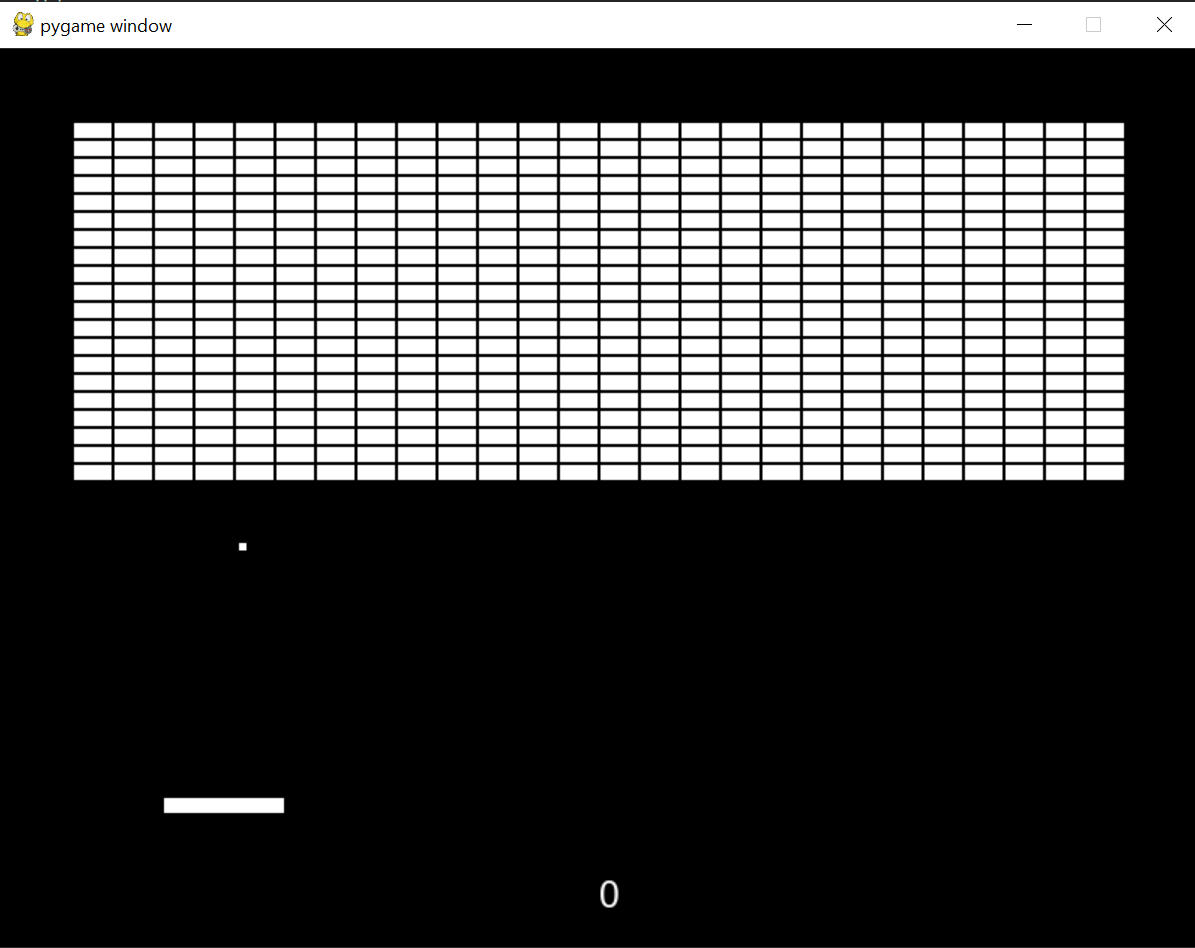
\includegraphics[scale=0.2]{layout0}
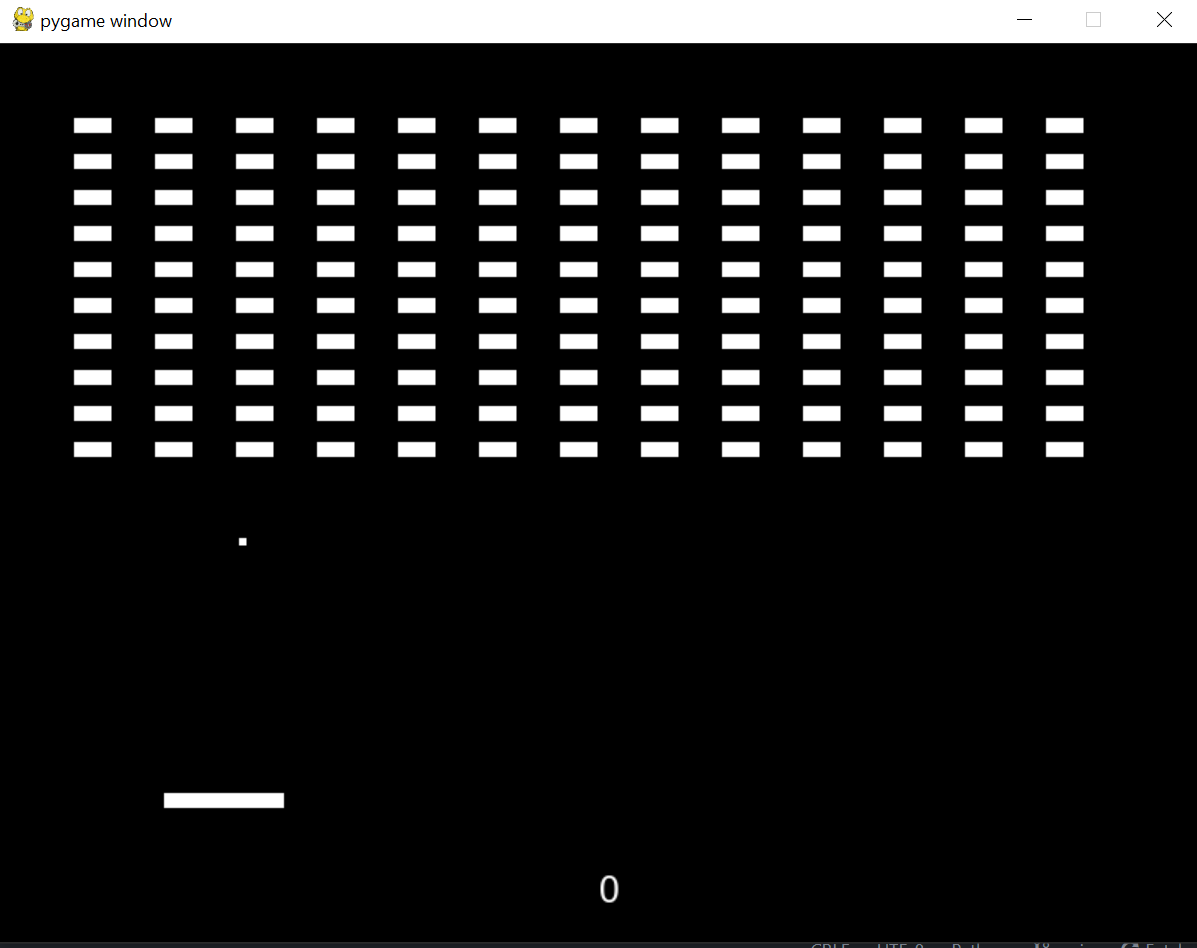
\includegraphics[scale=0.2]{layout1}
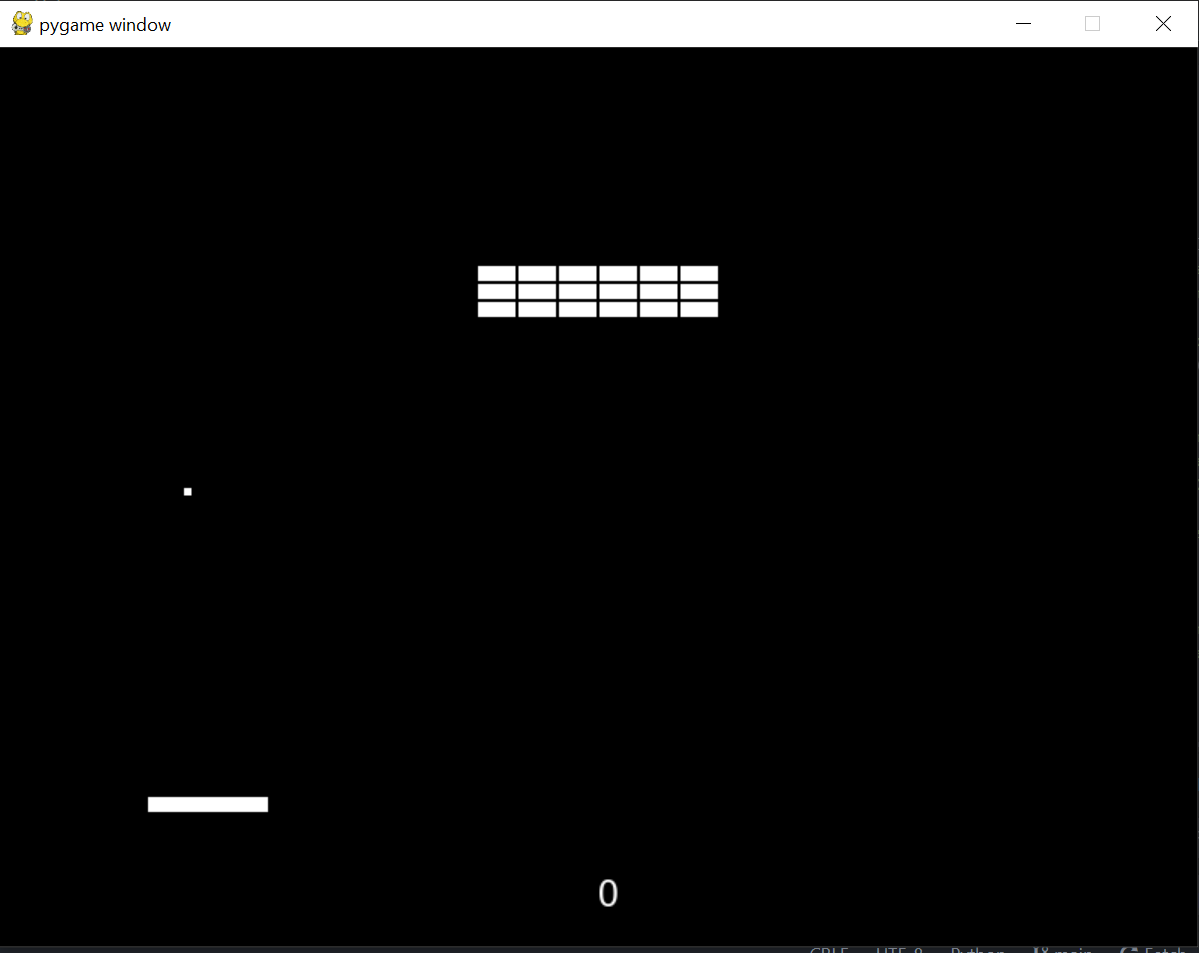
\includegraphics[scale=0.2]{layout2}
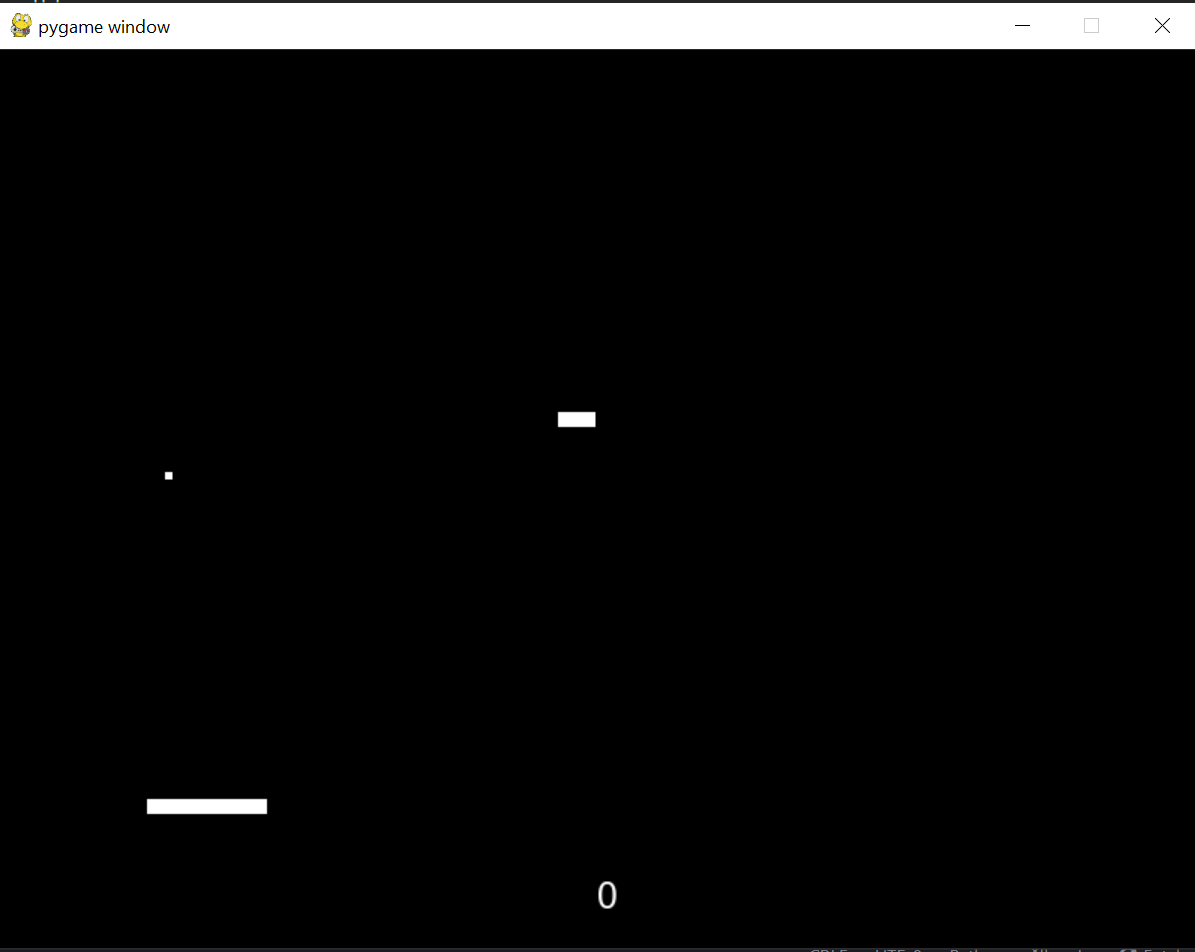
\includegraphics[scale=0.2]{layout3}
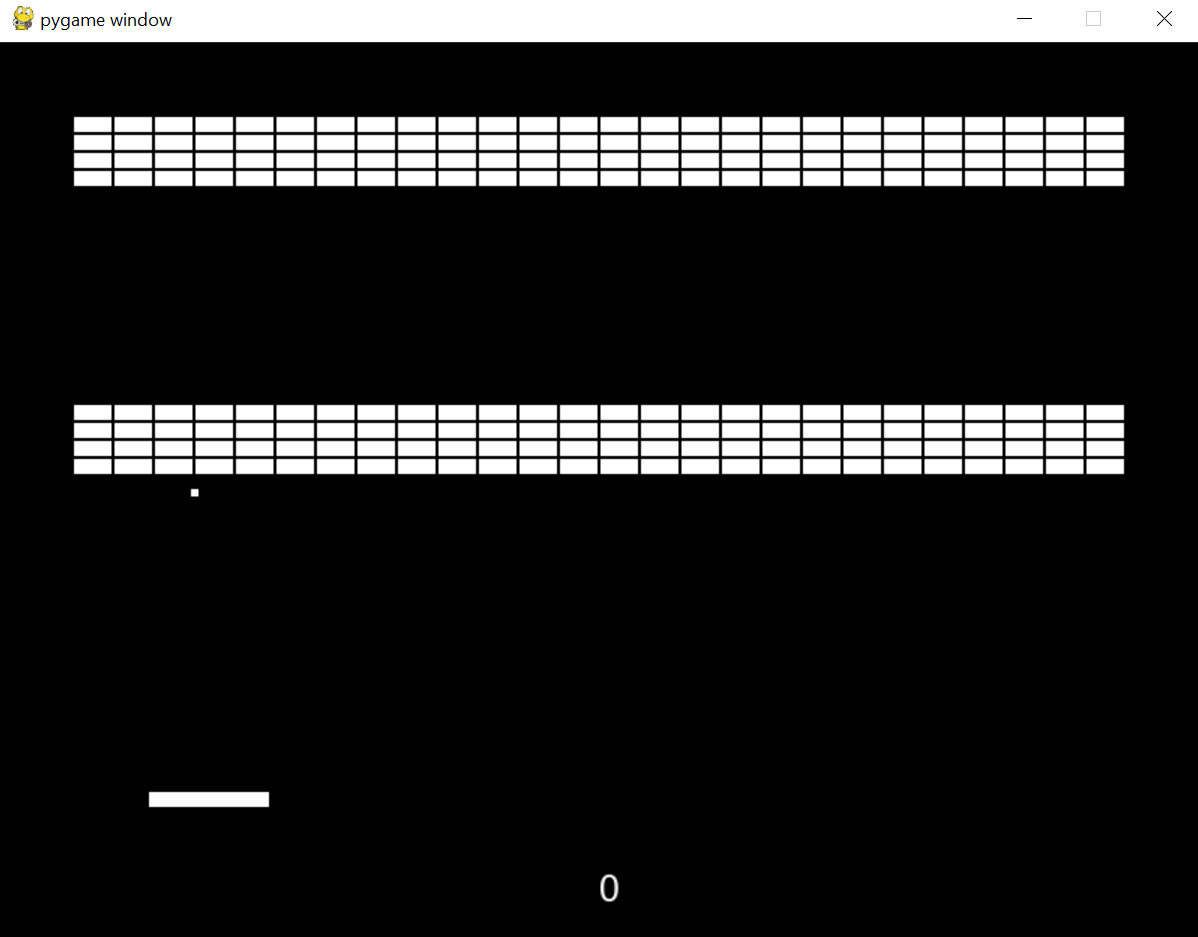
\includegraphics[scale=0.2]{layout4}
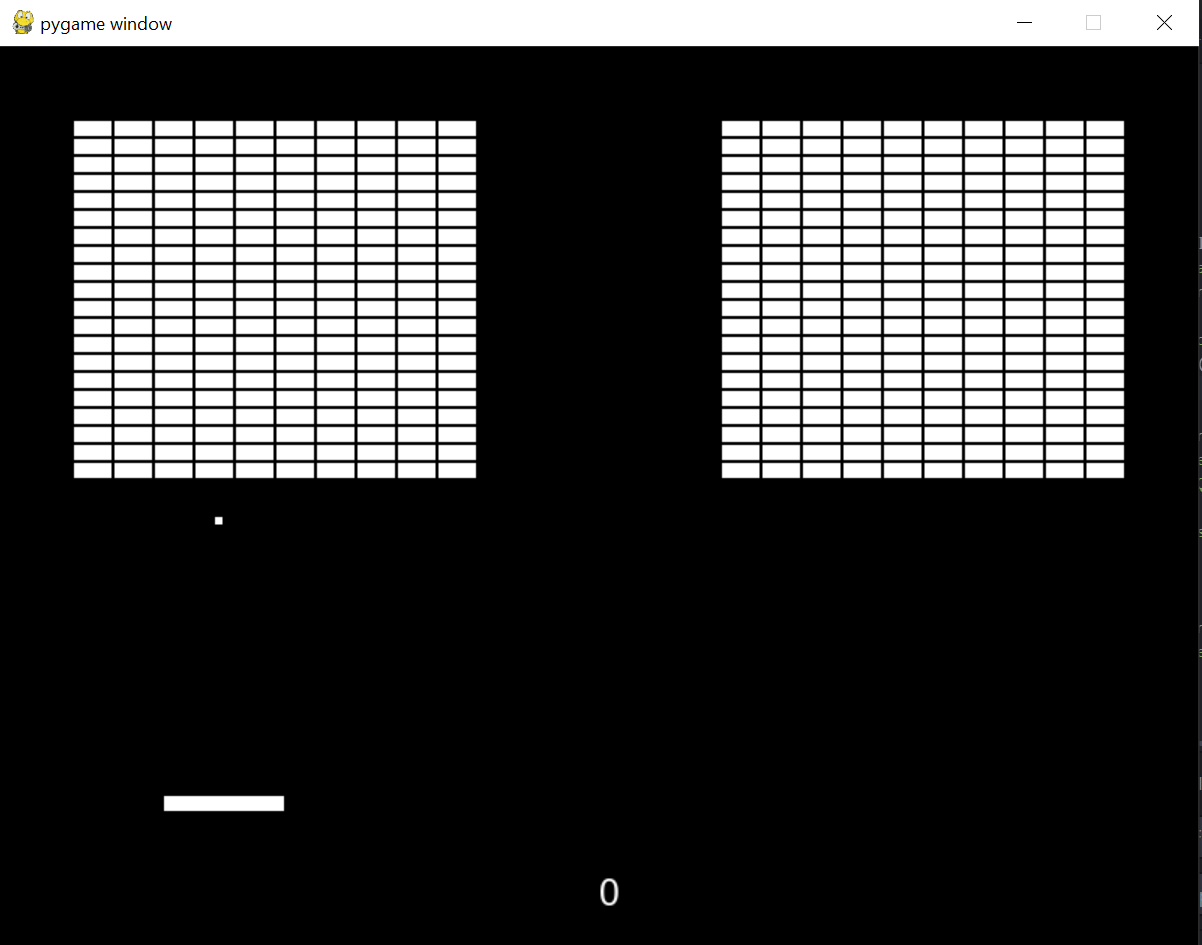
\includegraphics[scale=0.2]{layout5}
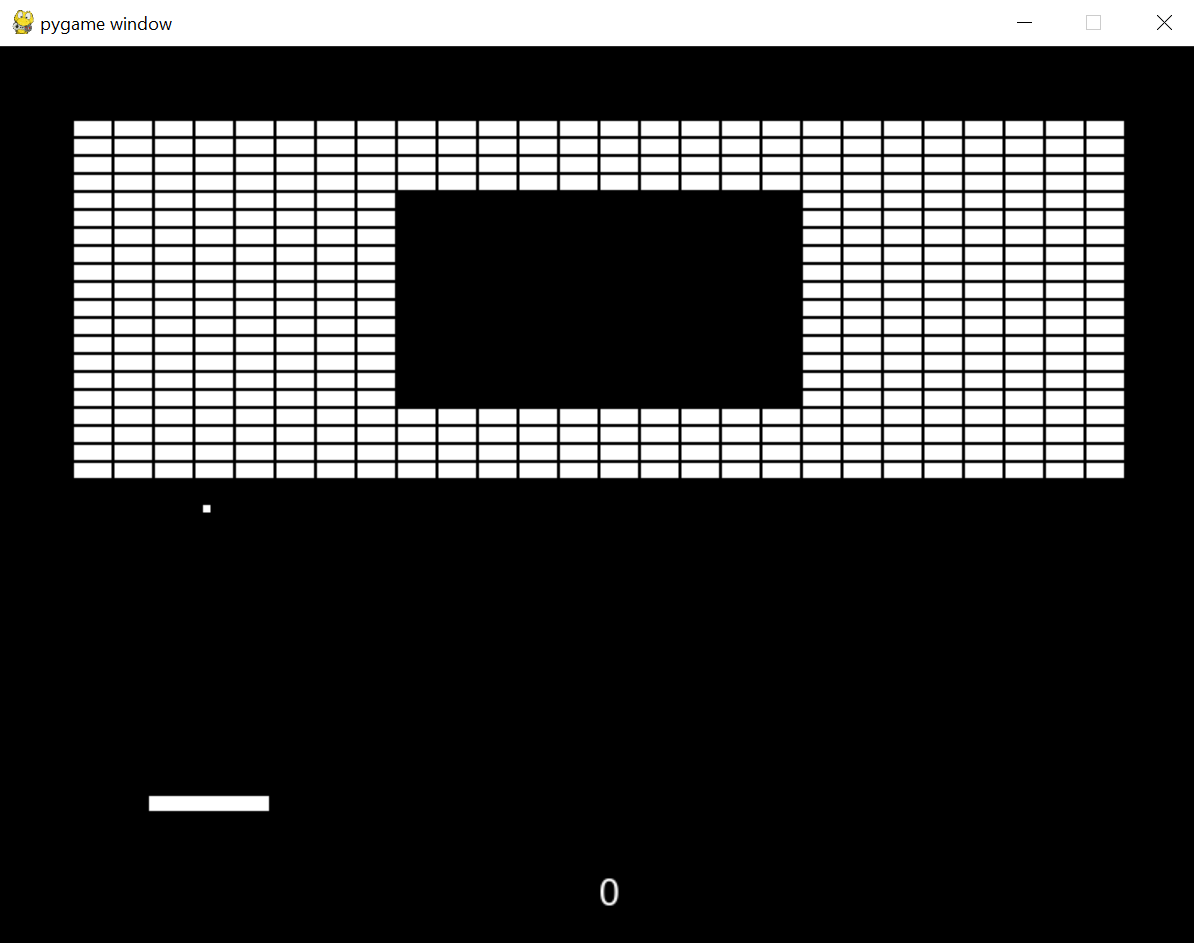
\includegraphics[scale=0.2]{layout6}
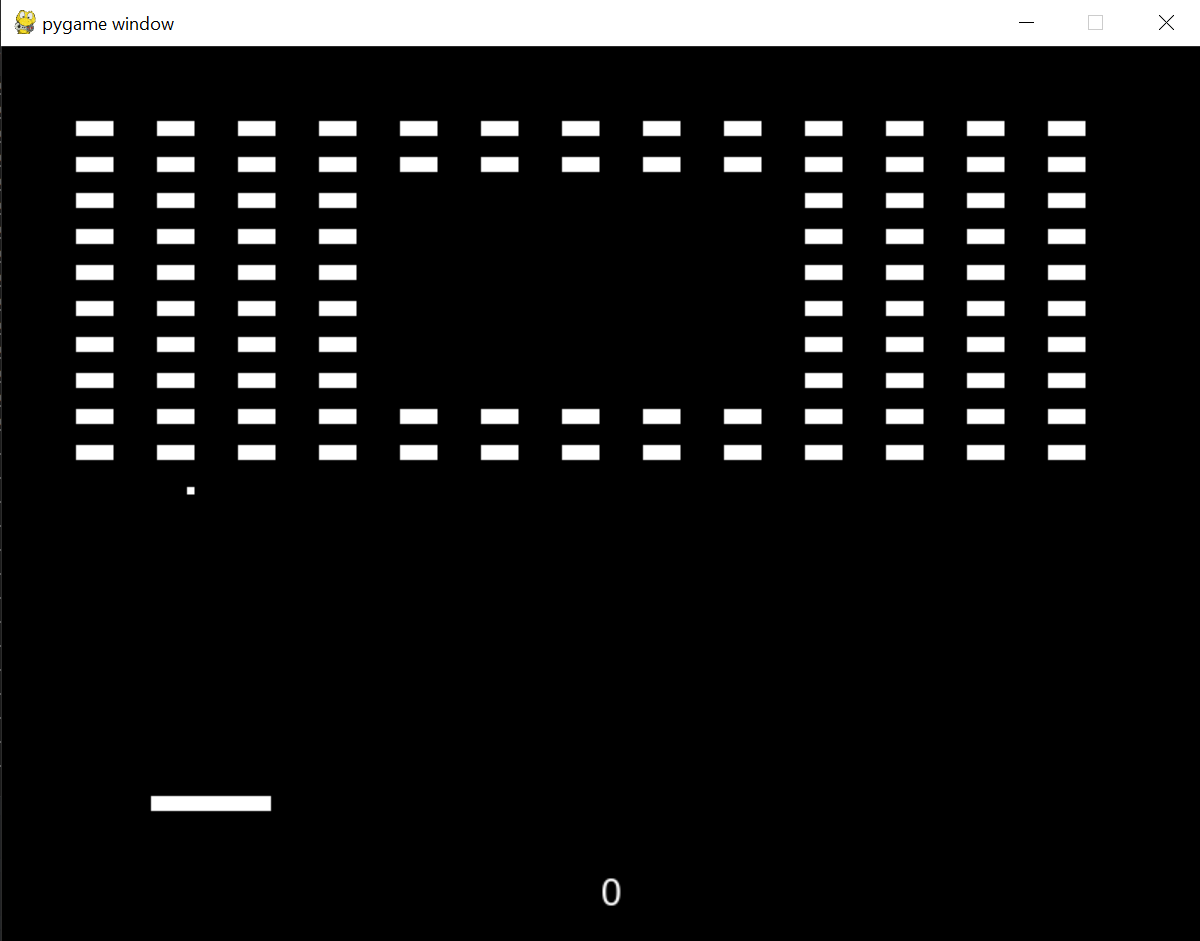
\includegraphics[scale=0.2]{layout7}
\centering
\end{figure}
The experiment we made to test generalization is \fnurl{here}{https://github.com/duoduocai-dot/csc498-project/blob/main/generalization_tests.py\#L10}. Essentially what it's doing is getting the trained agents from all 3 algorithms and running them across all layouts and measuring their score. Those algorithms were trained on layout1 (second layout in the top row). And along with them we included one more trained double Q-Learning agent which was trained for 100,000 episodes, and graphed the results. On the graph is also the max possible score achievable per layout as a reference to how well the algorithm does.
\begin{figure}[H]
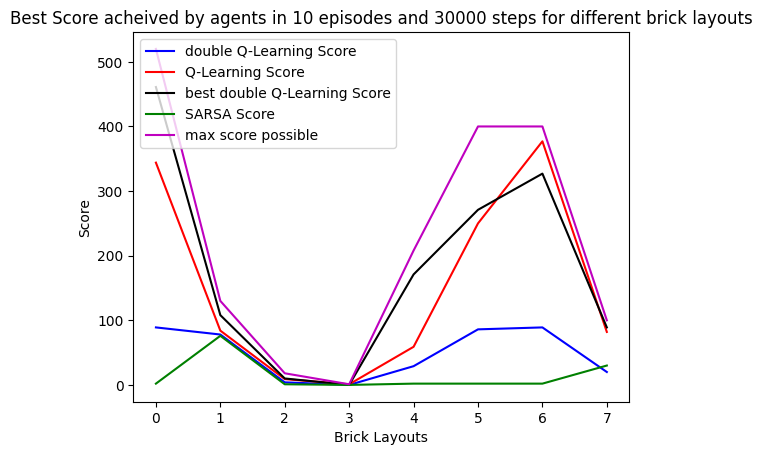
\includegraphics[scale=0.6]{BrickLayouts_generalization_tests}
\centering
\end{figure}
We can see both the Q-Learning and the best double Q-Learning algorithm do very well in generalizing across different layouts, both their scores are close the the maximum possible score.
\\\\
\fnurl{Here are example videos of the best double Q-Learning agent generalizing across brick layouts.}{https://github.com/duoduocai-dot/csc498-project/tree/main/pictures_and_videos/generalization_over_layouts}
\subsubsection{Which Layout is best to train on?}
We think that the layout best to train on is brick-layout number 1 (left). It is better than brick-layout 0 (right) because it allows for the ball to go in between bricks in a much earlier part of the episode than layout 0 allows. Thus the agent is able to learn more variations of ball locations and velocities.
\begin{figure}[H]
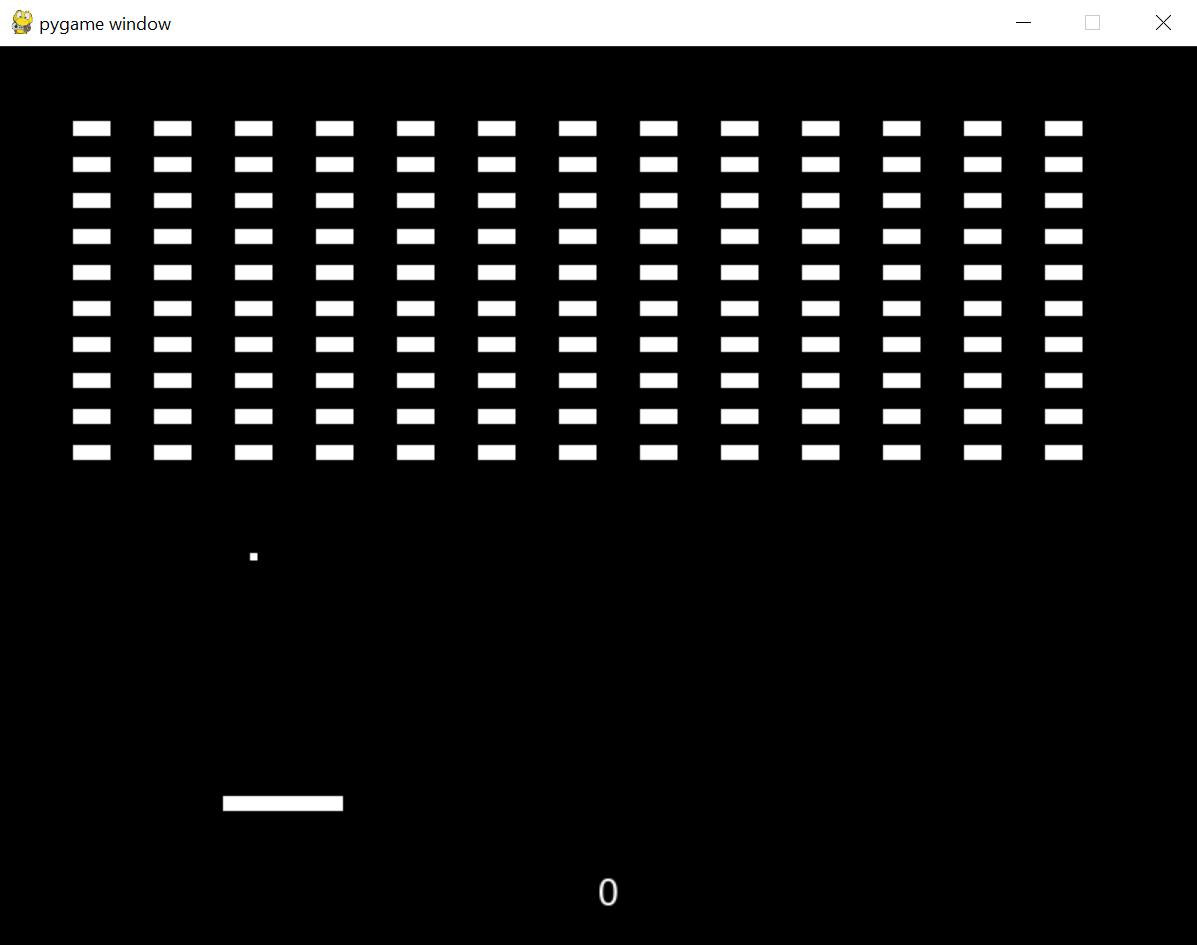
\includegraphics[scale=0.3]{bricklayout1}
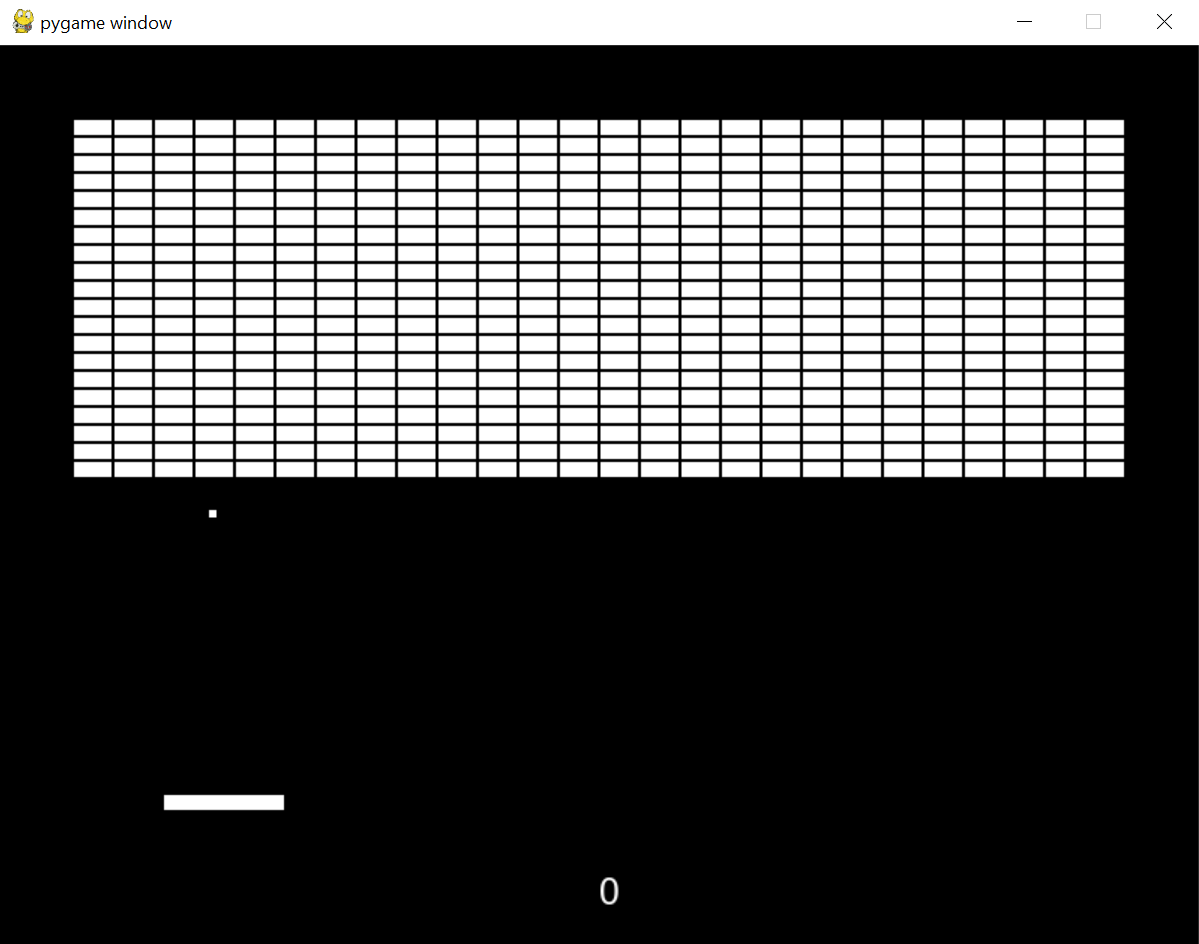
\includegraphics[scale=0.3]{bricklayout0}
\centering
\end{figure}

\subsection{Policy Gradient}
Our policy gradient implementation is \fnurl{here}{https://github.com/duoduocai-dot/csc498-project/blob/main/policy_gradient.py}. 
\subsubsection{Reward schema problems}
We had many issues with the initial reward schema in section 2.1. What was happening was that the agent was not moving. Essentially, the agent saw that any movement would result in lower reward, and  our learning rate was too high, such that the agent would get stuck in a gradient minimum. When we changed the reward schema to get close to the ball, the agent began learning.
\subsubsection{Gradients getting trapped}
Another problem with policy gradients that we were running into was the gradients getting stuck in a local min. 
\\\\We experimented a lot with the hyperparameters. Specifically, with the \fnurl{learning rate, we had some success by lowering it to be very small}{https://github.com/duoduocai-dot/csc498-project/blob/main/policy_gradient.py\#L55}, especially because our episode size was so large and as a result loss was very large. Another thing that helped with this problem was \fnurl{dividing loss by a large constant number}{https://github.com/duoduocai-dot/csc498-project/blob/main/policy_gradient.py\#L93}. However, even with all these changes the gradient still got stuck at random local minimas. Here is a video of a \fnurl{policy gradient agent playing the game}{https://github.com/duoduocai-dot/csc498-project/blob/main/pictures_and_videos/best_policy_gradient_agent.mkv}.
\\\\
Other things we tried to solve this problem was by including exploration. We added a greedy exploration in the algorithm, so the agent can get a feel for the environment, although it was unclear if this helped as the same problems above kept occurring. 
\\\\
Some other things we could try to fix this is by using momentum in the gradient update (\fnurl{although Adam optimizer used}{https://github.com/duoduocai-dot/csc498-project/blob/main/policy_gradient.py\#L55} should already be doing this). Another potential fix is to use the \fnurl{soft-actor critic algorithm}{https://arxiv.org/abs/1801.01290} which maintains stochasticity by having ample exploration. 

\subsection{Deep Recurrent Q-Network}
The deep recurrent Q-network has most of the ideas from the paper ..., to calulate the target function, we utilize a gated recurrent unit with one layer. Architecture: unidirectional, input size: 6 (observation space), one hidden layer of size 10, output size 3 (action space). In the forward pass, the computed value is then passed into a linear model. In the experience replay buffer, we sample sequences instead of single points.
\newline
The resaon we use GRU: \newline
\begin{itemize}
\item Given that the problem is relatively simple, using LSTM is inefficient.
\item The forget gate of LSTM is not useful in our case, because we don't need to skip any weak past frame and reuse them in later stages. 
\end{itemize}
\bibliography{bibliography}

\end{document}